\documentclass[a4paper, 12pt, UTF8]{article}

% preamble
% package
\usepackage{ctex}
\usepackage{geometry}
\usepackage{graphicx}
\usepackage{float}
\usepackage{caption}
\usepackage{enumerate}


% command
\graphicspath{{pic/}}
\geometry{
    textheight=230mm
}

\begin{document}

\title{\Huge 英译汉课程}
\author{\Large 
        第一周 第二周 \\[12pt]
        1931991 任家平 \\[12pt]
        同济大学 \\[12pt]
        测绘与地理信息学院}
\date{2019-09-11}
\maketitle

\thispagestyle{empty}

\newpage
\pagenumbering{Roman}
\tableofcontents
\addtocontents{toc}{\protect\vspace{10pt}}

\newpage
\pagenumbering{arabic}
\part{作业}

\newpage
\section{正文(部分)}

\begin{bfseries}
    \Large 
    Grand openings
    \paragraph*{}
    \large
    Changes that will bring scientific discovery more freely into the public domain are happening. About time too.
\end{bfseries}

\paragraph*{}
    IN 2001 a meeting on scientific publishing held in Budapest by what was then called the Open Society Institute (now the Open Society Foundation) coined the phrase “open access”. The gathering official statement asked the world to “share the learning of the rich with the poor and the poor with the rich, make this literature as useful as it can be, and lay the foundation for uniting humanity in a common intellectual conversation” --- in other words, to make scientific papers free to users.

\paragraph*{}
    A noble aspiration, but one which cynics might have thought had little chance of coming to fruition. The rich, they would observe, include academic publishers, who have enjoyed three centuries of dominion over the dissemination of scientific work and who often have profit margins approaching 40\%. They had every incentive to scupper change.

\paragraph*{}
    Cynicism, however, is not always correct. The open-access movement which the meeting helped spawn now looks unstoppable. All seven of Britain’s research councils, for example, now require that the results of the work they pay for are open-access in some way. So does the Well-come Trust, a British charity whose medical-research budget exceeds that of many scientifically successful countries. And by 2016 every penny of public money given to British universities by the government will carry the same requirement.

\paragraph*{}
    Elsewhere, the story is the same. In 2013, after years of wrangling in America’s Congress, the White House stepped in to require federal agencies that spend more than \$100m a year on research to publish the results where they can be read for free. Countless universities, societies and funding bodies in other countries have similar requirements.

\newpage
\section{第一版}
\subsection{翻译}
\begin{figure}[H]
    \centering
    \includegraphics[width = \textwidth]{original_work_01.jpg}
    \caption{第一版翻译\_01}
    \label{Fig:1}
\end{figure}

\newpage
\begin{figure}[H]
    \centering
    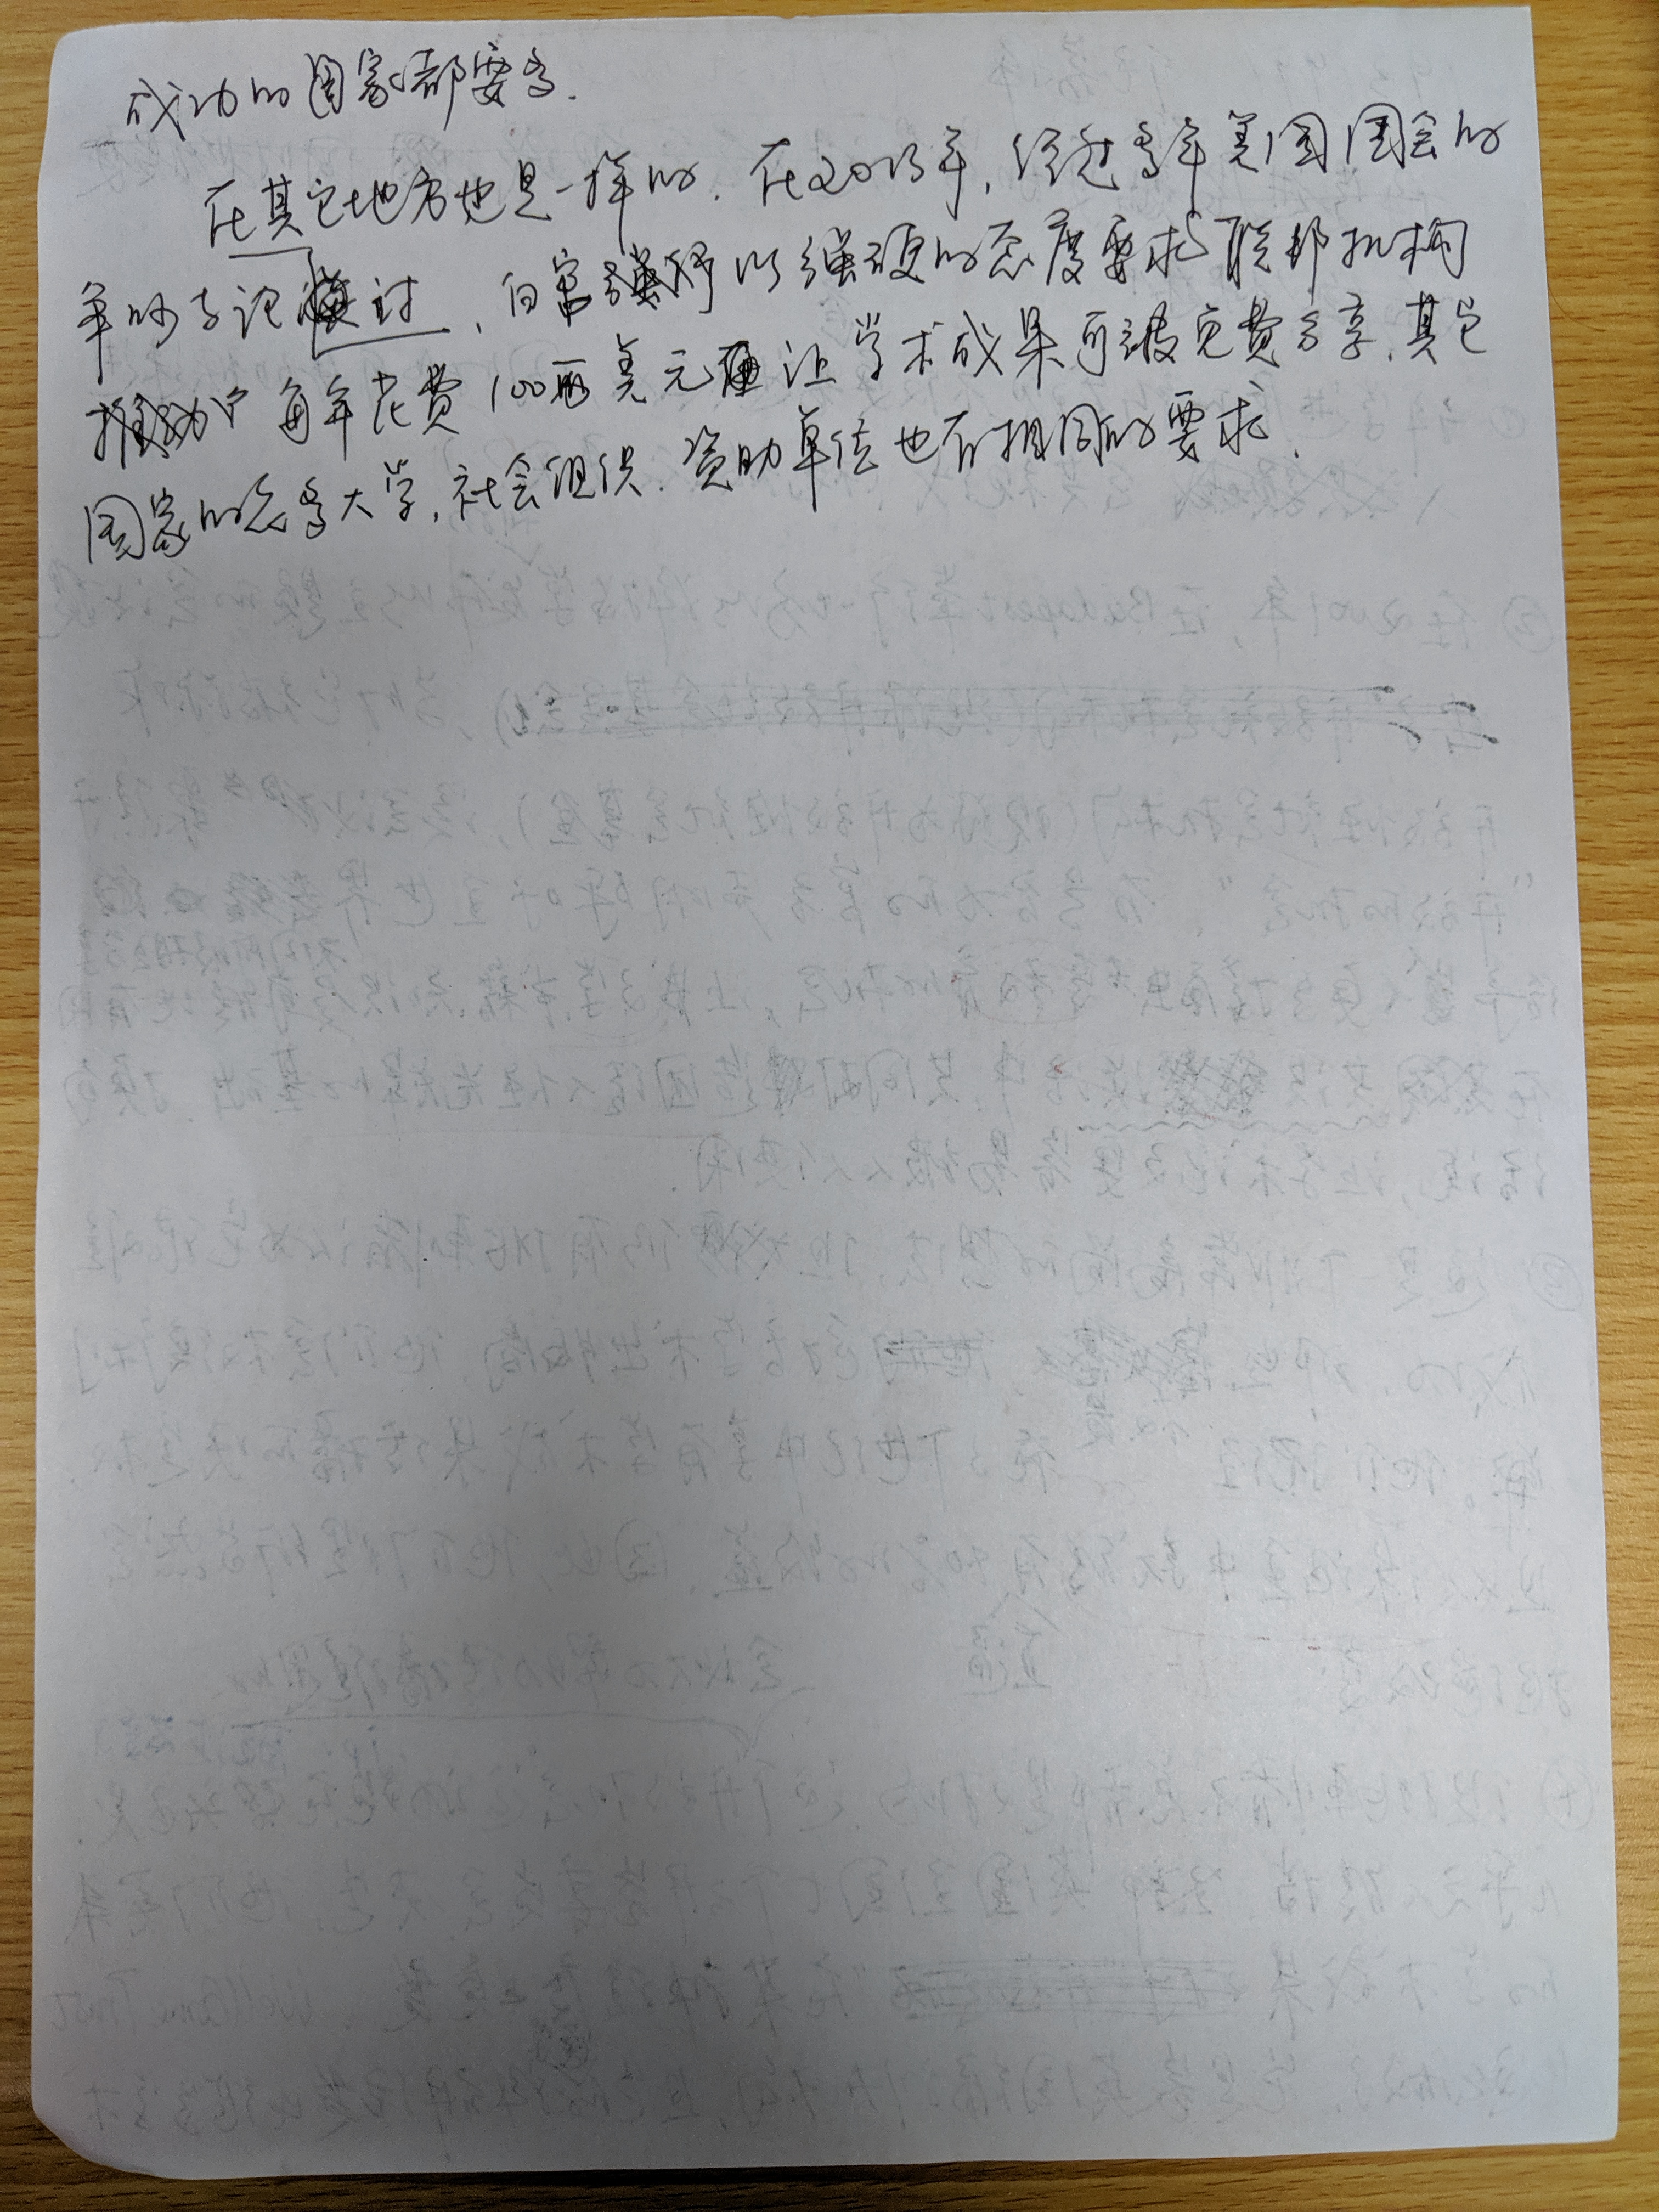
\includegraphics[width = \textwidth]{original_work_02.jpg}
    \caption{第一版翻译\_02}
    \label{Fig:2}
\end{figure}

\subsection{反思}
\begin{enumerate}[\hspace{0.5cm} 1.]
    \item {\bfseries public domain} 公共领域
          \begin{itemize}
              \item \emph{我的翻译:} 公共视线
              \item 一开始我翻译的是\lq 公共领域 \rq\ , 然后又改成了\lq 公共视线 \rq. 这说明我自己其实也不知道怎么翻译, 还是因为见的太少.
          \end{itemize}
    \item {\bfseries About time too.} It's about time to make this change too.
          \begin{itemize}
              \item \emph{我的翻译:} 对比上文中的 \lq more freely\rq\ 将其翻译成\lq 更快\rq. 在课堂上又思考了稍许, 将其与 \lq time that ... is happening\rq\ 作对比, 译作\lq 时代\rq. 
              \item 统统都不对, 这句话更偏向是口语中的\lq 是时候了\rq. 还是见的太少. 
          \end{itemize}
    \item {\bfseries the learning of ...} 知识, 科学刊物
          \begin{itemize}
              \item \emph{我的翻译:} 受教育
              \item 抽象地太多. 翻译的时候更应注重上下文的衔接.
          \end{itemize}
    \item {\bfseries literature} 论文, 知识
          \begin{itemize}
              \item \emph{我的翻译:} 文学
              \item 千万不能直译, 一定要联系上下文.
          \end{itemize}
    \item {\bfseries common intellectual conversation} 学术交流
          \begin{itemize}
              \item \emph{我的翻译:} 共同智力会谈 
              \item 感觉在翻译的时候脑子乱掉了. 遇到这种第一遍不懂得东西, 理应去用上下文联想.
          \end{itemize}
    \item {\bfseries humanity} 人类
          \begin{itemize}
              \item \emph{我的翻译:} 人性
              \item 平时见到 humanity 基本都是人性, 所以没多想直接翻译成人性, 就有了很搞笑的人性光辉的翻译.
          \end{itemize}
    \item {\bfseries margins} 顶, 边
          \begin{itemize}
              \item \emph{我的翻译:} 保证金 
              \item \lq margin\rq\ 在中文有\lq 顶, 边\rq\ 的意思, 平时看英文也经常见到这个单词, 课堂上是真的慌了.
          \end{itemize}
    \item {\bfseries spwan} 产生
          \begin{itemize}
              \item \emph{我的翻译:} 传播
              \item 脑子里对很多词的意思都是模糊的, 只记了个大概. 所以就翻译错了.
          \end{itemize}
\end{enumerate}

翻译的很差, 关键点都是乱翻的. 自己觉得全文的难点就在于概述和第一段. 如\lq common intellectual conversation\rq\ 很考验译者理解能力, 具体表现在联系上下文的能力. 同时也启发我, 有时候碰到这种高上大的名词, 如果直译的意思完全沾不上边, 就应该去发挥自己想象力, 因为这个短语极可能与文章或是报道的主题有关系. 算是一种翻译技巧. 

同时看的东西少, 也缺乏很多翻译的自信, 会犹豫不决, 甚至会改变业界的惯性翻译, 这在专业人士眼里会显得十分业余且可笑. 总而言之, 不专业, 也正正好好符合自己业外人士的身份.

所以显得十分真实.

\newpage
\section{第二版}
\subsection{翻译}
学术进展的新发现将更容易进入公共领域, 也是时候做出这样的改变了.

2001年, 在 Budapest 举行了一场以学术刊物发表为主题的会议, 当时它被称作开放社会研究所(现在被称作开放社会基金). 在这个会议上提出了\lq 开放获取\rq\ 的概念. 这个具有号召力的官方声明呼吁全世界间不同阶级相互分享, 更应让社会底层拥有接触学术文献的机会, 让文献尽其所用, 这为之后人类的学术交流打下了坚实的基础. 换句话说, 让学术刊物更容易被大众使用.

这是一个十分崇高的理念. 但仍有不少挑刺者认为它不可能实现. 那些包括学术出版商在内的权贵们, 他们会权衡利弊, 因为他们已经在三个世纪中享有学术成果的传播决定权, 并从中获取逼近40\%的利益. 因此, 他们理所当然会拒绝改变.

然而这些挑刺者不总是对的. 这个被会议促成的\lq 开放获取\rq\ 运动无人能挡. 比如, 英国全部七个研究委员会要求他们的学术成果在某种程度上免费获取. Well-come Trust是一家英国的慈善机构. 它的医学研究预算已经超过了多个科学发达国家. 在2016年之前, 有英国政府补助的科研结果也应该免费向大众开放.

其他地方情况也差不多. 在2013年, 经过美国国会多年的激烈讨论, 白宫介入, 要求联邦机构每年多花100万美金去让科技成果文献免费为大众开放. 其他国家很多的大学, 社团和基金都如此要求.

\subsection{反思}
这回在翻译前, 好好把各种名词查了一遍, 所以条理更加清晰. 比如\lq Open Society Institute\rq (开放社会研究所)和 \lq open access\rq (开放获取)的翻译, 这种词汇应该是有公认的翻译, 但如果第一次翻译, 不去上网查找资料, 很容易就会翻译出\lq 别名\rq (开放社会机构, 开放机会). 不知道这种情况在专业的翻译中, 是否允许. 在翻译的同时, 也对第一次翻译的错误进行了纠正, 译文读起来就流畅了许多.

翻译的核心还是要理解整个文章内容. 如果是我自己做的话, 肯定有很多地方翻译不到位. 也正巧有了这节课的点拨, 对于文章难点部分如何理解翻译, 提供了新的方法与思路. 同时自己也要注意翻译的态度, 要把它当做自己的一份作品而非草稿去完成, 态度要摆端正, 不能因为自己是业外人士就嘻嘻哈哈, 降低要求. 课下也应该多看看 NY Times 或是 Guardian 这类的报纸.

之前买了几本上海高口的教材, 虽然老师点评证书的含金量不高, 但是阅读教程里的大部分文章质量很高. 我也花了两个星期大概把第一章里的文章过了一遍, 仍然有很多地方不懂, 课上也给了我一些关于翻译方法的启发, 希望能靠自己把问题解决.

接下来对文章的某些句子的翻译记录一下想法. 在第一版反思中提到的在此不赘述.

\begin{enumerate}[\hspace{0.5cm} 1.]
    \item scientific \\
          不应为\lq 科技\rq, 在本文中译为\lq 学术\rq\ 更为贴切.
    \item rich, poor\\
          如果两者在\lq and\rq\ 前后出现, 可以一起译作\lq 不同阶级\rq. rich单出现可译作\lq 权贵\rq, poor可译作\lq 底层\rq.同时要注意类似词语的词性, 因为它们是反义词, 只要翻译出其中一个, 可以根据反义词推出另一个. rich 在此广义指的是在科技文献获取机会上占优的一方, poor理所当然就成了在科技文献获取机会上劣势一方, 至于具体用中文的哪些词语代替 rich 和 poor 就是考察译者语文功底了.
    \item observe\\
          根据上下文, 译作\lq 权衡利弊\rq. 全文主题是开放获取, 科技文献免费对公众开放, 那么利益受损的必然是权贵们. 这就是看懂文章核心内容之后的逻辑. 后面的一系列定语从句, 看上去虽是对权贵的描述, 但结合本段第一句, 这些定语从句描述的是为什么挑刺者会对运动会抱有悲观的解释. 这就是这一段的逻辑结构. oberseve, 直译是观察, 开放运动掀起, 权贵们在观察, 这么翻译不通顺, 因此译为思考或是观望更为准确, 思考什么呢? 思考运动开始, 自己获利减少, 为了保持自己利益不变, 所以要拒绝改变, 拒绝这场开放获取运动, 即observe本质是为了利益, 把 思考, 利益, 观望 放在一起, 权衡利弊呼之欲出.
    \item \lq by 2016 ... same requirement\rq \\
          没有直译, 在这里 \lq every penny of ...\rq\ 直译是\lq 英国政府在科研上投入的每一分钱\rq. 如果直译就成了, 英国政府在科研上投入的每一分钱也要遵守同样的要求. 显得很奇怪, 这里\lq 同样的要求\rq 指的是上文所说免费向大众开放. 那么\lq 英国政府在科研所投入的钱\rq\ 就可以理解为有英国政府补助过的或是经过英国政府资助的科研成果. 因此整个句子翻译为\lq 有英国政府补助的科研结果也应该免费向大众开放\rq. 
    \item \lq on research ... for free\rq \\
          同上, 不能直译, 直译后的句子很不流畅.
\end{enumerate}

\newpage
\part{补充性材料}

\newpage
\section{正文(全文)}
\begin{bfseries}
    \Large
    Grand openings
    \paragraph*{}
    \large
    Changes that will bring scientific discovery more freely into the public domain are happening. About time too.
\end{bfseries}

\paragraph*{}
    IN 2001 a meeting on scientific publishing held in Budapest by what was then called the Open Society Institute (now the Open Society Foundation) coined the phrase “open access”. The gathering official statement asked the world to “share the learning of the rich with the poor and the poor with the rich, make this literature as useful as it can be, and lay the foundation for uniting humanity in a common intellectual conversation” --- in other words, to make scientific papers free to users.

\paragraph*{}
    A noble aspiration, but one which cynics might have thought had little chance of coming to fruition. The rich, they would observe, include academic publishers, who have enjoyed three centuries of dominion over the dissemination of scientific work and who often have profit margins approaching 40\%. They had every incentive to scupper change.

\paragraph*{}
    Cynicism, however, is not always correct. The open-access movement which the meeting helped spawn now looks unstoppable. All seven of Britain’s research councils, for example, now require that the results of the work they pay for are open-access in some way. So does the Well-come Trust, a British charity whose medical-research budget exceeds that of many scientifically successful countries. And by 2016 every penny of public money given to British universities by the government will carry the same requirement.

\paragraph*{}
    Elsewhere, the story is the same. In 2013, after years of wrangling in America’s Congress, the White House stepped in to require federal agencies that spend more than \$100m a year on research to publish the results where they can be read for free. Countless universities, societies and funding bodies in other countries have similar requirements.

\paragraph*{}
    Publishers, though they have often dragged their feet, are adjusting. This week the oldest, the Royal Society, and arguably the most prestigious, Nature Publishing Group (NPG)—both based in London—joined in. Each will now publish a journal that readers do not have to pay to look at.

\paragraph*{}
    \begin{bfseries}
        \large
        Who will publish, and who perish?
    \end{bfseries}

\paragraph*{}
    Open-access publishing actually began in 2000, a year before the Budapest meeting, with the launch, in Britain, of BioMed Central, and in America, of the Public Library of Science (PLOS). The open-access business model shifts the cost of producing the journal from subscribers, such as university libraries, to researchers themselves, who pay an article-processing charge (APC) to appear in print or its electronic equivalent. Either way, the taxpayer picks up the bill in the end. But open publication makes research more widely accessible, which is a public good in its own right.

\paragraph*{}
    One problem open access brings is a shift in incentives. More published articles means more revenue from processing charges. Rejection rates at high-end paid-for journals often exceed 90\%. A commercial open-access publisher (which PLOS, a charity, is not) might be tempted to publish anything that came his way, in order to pocket the APC—and many have, giving open access a fly-by-night feel to some academics.

\paragraph*{}
    For example, in a survey conducted by NPG, of 27,000 authors of papers in its journals, 44\% expressed some concern about the quality of open-access publishing and more than a third agreed with the notion that it was associated with less prestige. Yet those perceptions may be misguided. A study of Nature Communications (which was, until this week’s announcement, a hybrid between open access and traditional subscription, but is now pure open access) shows that its open-access papers enjoyed a slightly higher number of citations and significantly more downloads and online views than their non-open-access brethren.

\paragraph*{}
    To foster prestige, champions of open access have launched efforts such as eLife, an online journal with an array of academic bigwigs at its helm. They hope to create a top-tier publication by sheer weight of bigwiggery. But eLife and its kind cannot force the change alone, because publishing with the requisite due diligence is not cheap.

\paragraph*{}
    The Public Library of Science has found a way out of this by copying the more-the-merrier approach, but in a controlled way. Until 2006 it was a producer of high-impact but loss-making publications. Then it started PLOS ONE, a different kind of journal altogether. Instead of acting as an arbiter of the importance of scientific work, PLOS ONE claims only to ensure that articles are scientifically sound. With less effort going into peer review, PLOS ONE publishes many more papers (in 2013, it carried more than 31,000 articles, 36 times as many as the next-most-prolific PLOS journal) while simultaneously charging less for them and becoming a cash-cow that helps pay for the rest of the outfit. The Royal Society hopes to recapitulate this idea with its new offering, Royal Society Open Science.

\paragraph*{}
    \begin{bfseries}
        \large
        Free hits
    \end{bfseries}

\paragraph*{}
    Whether the experience of Nature Communications will overcome researchers’ misgivings remains to be seen. Despite the Wellcome Trust’s requirement that its grantees publish in open-access journals, only 70\% do so. To ensure compliance, the trust has had to introduce punitive measures, such as withholding money.

\paragraph*{}
    Some researchers just don’t care, though. A survey by Taylor \& Francis, a publishing firm, asked American and British scientists if they had published under open-access policies; 44\% and 32\%, respectively, did not know. More than half responded they did not know if they would in future. But many do know, and resist.

\paragraph*{}
    The point about prestige is not mere snobbery. The league table of journals is as finely graded as that of football, and, at the moment, has far less scope for promotion and demotion. Grant-awarding bodies and appointment committees know this and, in a wonderful display of doublethink, promote open access but also promote those who eschew it by publishing in top-notch, non-open journals

\paragraph*{}
    Only when that changes will open access’s victory be complete. This could happen either by new open-access journals acquiring the necessary kudos, or by old ones, seeing the game is up, becoming open access themselves. Though Nature Communications is a successful and well-regarded publication, it is not NPG’s top product. And Royal Society Open Science is untested. At the moment, then, both the Royal Society and NPG seem to be hedging their bets. When the society’s Proceedings, and NPG’s eponymous flagship, Nature, are both free for anyone to read, then open access’s partisans really will be able to declare victory and go home.

\paragraph*{}
    \emph{\small The Economist, Sep 27th, 2019}

\section{翻译}
学术进展的新发现将更容易进入公共领域, 也是时候做出这样的改变了.

2001年, 在 Budapest 举行了一场以学术刊物发表为主题的会议, 当时它被称作开放社会研究所(现在被称作开放社会基金). 在这个会议上提出了\lq 开放获取\rq\ 的概念. 这个具有号召力的官方声明呼吁全世界间不同阶级相互分享, 更应让社会底层拥有接触学术文献的机会, 让文献尽其所用, 这为之后人类的学术交流打下了坚实的基础. 换句话说, 让学术刊物更容易被大众使用.

这是一个十分崇高的理念. 但仍有不少挑刺者认为它不可能实现. 那些包括学术出版商在内的权贵们, 他们会权衡利弊, 因为他们已经在三个世纪中享有学术成果的传播决定权, 并从中获取逼近40\%的利益. 因此, 他们理所当然会拒绝改变.

然而这些挑刺者不总是对的. 这个被会议促成的\lq 开放获取\rq\ 运动无人能挡. 比如, 英国全部七个研究委员会要求他们的学术成果在某种程度上免费获取. Well-come Trust是一家英国的慈善机构. 它的医学研究预算已经超过了多个科学发达国家. 在2016年之前, 有英国政府补助的科研结果也应该免费向大众开放.

其他地方情况也差不多. 在2013年, 经过美国国会多年的激烈讨论, 白宫介入, 要求联邦机构每年多花100万美金去让科技成果文献免费为大众开放. 其他国家很多的大学, 社团和基金都如此要求.

出版商们并不想将学术刊物免费提供大众, 但外界压力逼得他们不得不做出改变. 这周在伦敦, 最老的学术出版商英国皇家学会和富有争议性的著名学术出版商自然杂志出版集团也加入了开放获取运动, 他们承诺会发布向公众免费的学术刊物.

\paragraph*{\large 谁出版? 谁苦逼?} \hspace{10pt} \\

开放获取运动其实早在 Budapest 会议一年之前的2000年就开始了. 当时是由英国的生物制药中心和美国的公共科学图书馆发起. 开放获取运动使学术出版的商业模式发生了改变, 之前由大学图书馆之类的订阅者来承担刊物的印刷费, 而现在由科研工作者付一笔出版费, 用于在学术期刊或其电子版上发表. 无论哪种商业模式, 最后还是由公众买单. 但相比之下, 开放获取运动还是更易让学术刊物被大众获取, 造福大众.

但开放获取运动带来的一个问题就是出版社刊登文章动机的转变. 现在出版社的营业收入与出版费挂钩, 刊登更多的论文意味着更高的收益. 高端付费的学术刊物对投稿者的拒绝率高达90\%. 参加开放获取运动的盈利性出版商可能经不起诱惑, 为了从出版费捞一笔, 别人投什么他就发什么, 这就会让一些不可靠低质量的论文被发表.

例如, 在自然杂志出版社集团的一个问卷中, 对自然杂志发表文章的27000名投稿人进行了调查, 44\%的人表达了对开放获取刊物中论文质量的担忧, 多于三分之一的人认为开放获取运动威望大打折扣. 然而这些投稿人的看法可能有点狭隘片面. 根据自然通讯的一个研究显示, 开放获取出版商的刊物引用量稍稍多于传统出版商刊物, 下载量和在线访问量要多得多.

为了维护名誉, 开放获取出版商中的佼佼者 eLife 做出了一系列改变. 它是一家以学术大佬撑腰的在线刊物. 它想仅凭学术大佬们的力量搞一个顶尖刊物. 但毕竟这么干很花钱, 仅靠 eLife 单打独斗远远不够.

公共科学图书馆出版社创造出了一种质量有保证的薄利多销经营方式. 2006年之前, 它虽是一个有影响力的出版商, 但其实一直在亏钱. 之后它们发行了 PLOS ONE, 一个与众不同的刊物. PLOS ONE 不去要求论文的高质量, 只要不是粗制滥造就好. 这样可以大大减少同行审查的成本. 结果 PLOS ONE 文章刊登量显著提高. 在2013年, 它发表了31000多篇论文, 比第二多产的 PLOS 的36倍还要多. 与此同时, 向投稿者收的出版费比其他刊物少. 薄利多销, PLOS ONE 变成了公共科学图书馆的摇钱树, 把 PLOS 部分的亏损也补上了. 皇家学会也想这么搞, 于是推出了皇家学会开放学术.

\paragraph*{\large 运动受挫} \hspace{10pt} \\

自然通讯的调查结果能否打消学者们的顾虑仍是未知. 尽管 Wellcome-Trust 要求它的被资助人在开放获取的刊物上发表文章, 也只有70\%的人这么做. 为了达到这一目的, Wellcome-Trust 不得不弄出来一套扣钱之类的惩罚措施来确保被资助者在开放获取刊物上发表论文.

尽管如此, 还是有学者根本不在乎是否一定要在开放获取刊物发文章. 泰勒弗朗西斯出版公司对英美学者是否在开放获取的刊物发表过文章做了调查, 44\%的美国学者和32\%的英国学者表示自己根本都不知道还有开放获刊物取这种东西. 一多半人不清楚将来会不会参与开放获取运动. 受调查的很多学者知道开放获取运动, 但持抵制态度.

开放获取刊物的名望不仅仅是钱这种比较世俗的东西, 学术刊物的地位也对名望有极大影响. 不同学术刊物地位的排名和足球球队积分表排名有相似之处, 往往比较固定, 几乎没有上升或是下降的可能. 政府的拨款机构和提名委员会对此心知肚明, 他们鼓吹开放获取刊物的同时, 也在暗中提拔那些不参加开放运动的顶尖学术刊物. 真是一场完美绝伦的双标秀.

只有开放获取刊物的地位真正被政府机构和提名委员会认可, 开放获取运动才会迎来完整的胜利. 要么现有的开放刊物获取了足够的认可, 要么传统的不开放刊物见大势已去, 也变成了开放刊物. 尽管自然通讯很成功且学术地位相对较高, 但它并不是自然杂志出版社集团最拿手的刊物. 皇家学会开放学术还没有经得起时间的考验, 是个未知数. 现在看来, 皇家学会和自然杂志出版社集团想及时止损, 不想花大量精力做开放获取刊物. 大概只有当海军的 Proceedings 杂志和与自然杂志出版社集团齐名王牌刊物 Nature 全都免费开放时, 开放获取运动才真的成功, 它的铁杆粉丝们就能凯旋而归了.


\section{文章总结}
文章第一部分大致介绍了开放获取运动的形成和横扫全球的势头, 中间稍提了出版商的利益问题. 

在第二部分开始对利益分配做出了一些介绍. 具体为开放获取的商业模式的转换, 由此引出为公众带来福利的同时其本身存在的问题---低质量论文. 针对这一现象, 再引出学者的对其态度, 以及部分开放获取刊物为了反击低质量论文, 维护自己名誉而做出的努力. 

文章第三部分对第二部分中学者态度部分进行扩展, 再次将主题拉回学术刊物地位, 讲解学术刊物地位的决定性因素. 不仅仅是刊物能否盈利, 被大众认可, 更需要政府部门和委员会的认可. 然而他们的双标貌似让作者气愤. 

作者写道, 开放获取运动获取胜利的方式有两种, 一是现有的开放刊物获取了足够的认可, 二是传统的不开放刊物见大势已去, 也变成开放刊物. 但在最后一段, 作者对新兴的开放刊物的悲观显而易见, 有写到只有当两大付费刊物向公众开放时, 开放获取运动才能迎来真正的胜利, 由此可见, 作者还是对第二种方式更抱有信心.

\section{翻译感想}
翻译的挺累, 仍有一些不懂得地方需要请教. 

不过在翻译过程中慢慢体会到一些技巧性的东西. 之前自己看英文文章, 总是盯着几个不懂得词语纠缠不清, 因为潜意识里面还是想去直译, 包括我第一周课堂上的翻译, 也是直译. 现在觉得这种翻译意识很业余. 翻译的过程应该是, 从英文读懂文章在讲什么, 在脑子里形成自己理解的概念, 同时结合英文的关键字, 用中文再自己重新组织一遍. 以这种意识去翻译, 颇有种柳暗花明之感.

打算把之前看到的好文章就像这次作业一样过一遍. 拒绝眼高手低.
\end{document}